\documentclass[a4paper,10pt]{article}

%Math
\usepackage{amsmath}
\usepackage{amsfonts}
\usepackage{amssymb}
\usepackage{amsthm}
\usepackage{ulem}
\usepackage{stmaryrd} %f\UTF{00FC}r Blitz!

%PageStyle
\usepackage[german]{babel}
\usepackage{fontenc}
\usepackage{fancyhdr, graphicx}
\usepackage{wasysym}
\usepackage{fullpage}
\usepackage{textcomp}
\usepackage{fancyhdr} %for header/footer


\usepackage{wrapfig}
\usepackage{listings}

%My Commands
\newcommand{\BN}{\mathbb{B}} %BOOL
\newcommand{\RN}{\mathbb{R}} %Real Number
\newcommand{\NN}{\mathbb{N}} %Natural Number
\newcommand{\QN}{\mathbb{Q}} %Rational Number
\newcommand{\ZN}{\mathbb{Z}} %ganze Zahlen
\newcommand{\CN}{\mathbb{C}}
\newcommand{\Teilt}{\setminus} %\
\newcommand{\Teiltn}{\nmid} %kein teiler
\newcommand{\Potp}{\mathcal{P}} %Potenzmenge
\newcommand{\Pota}{\mathcal{A}}
\newcommand{\Potr}{\mathcal{R}}
\newcommand{\Potn}{\mathcal{N}}
\newcommand{\Bold}[1]{\textbf{#1}} %Boldface
\newcommand{\Kursiv}[1]{\textit{#1}} %Italic
\newcommand{\T}[1]{\text{#1}} %Textmode
\newcommand{\Nicht}[1]{\T{\sout{$ #1 $}}} %Streicht Shit durch
\newcommand{\lra}{\leftrightarrow} %Arrows
\newcommand{\ra}{\rightarrow}
\newcommand{\la}{\leftarrow}
\newcommand{\lral}{\longleftrightarrow}
\newcommand{\ral}{\longrightarrow}
\newcommand{\lal}{\longleftarrow}
\newcommand{\Lra}{\Leftrightarrow}
\newcommand{\Ra}{\Rightarrow}
\newcommand{\La}{\Leftarrow}
\newcommand{\Lral}{\Longleftrightarrow}
\newcommand{\Ral}{\Longrightarrow}
\newcommand{\Lal}{\Longleftarrow}
\newcommand{\Vektor}[1]{\vec{#1}}
\newcommand{\Brace}[1]{\left( #1 \right)} %()
\newcommand{\Bracel}[1]{\left\lbrace #1 \right.} %(
\newcommand{\Bracer}[1]{\right. #1 \right\rbrace} %)
\newcommand{\Brack}[1]{\left\lbrace #1 \right\rbrace} %{}
\newcommand{\Brackl}[1]{\left\lbrace #1 \right.} %{
\newcommand{\Brackr}[1]{\right. #1 \right\rbrace} %}
\newcommand{\Result}[1]{\underline{\underline{#1}}} %Doppelt unterstrichen
\newcommand{\Abs}[1]{\left| #1 \right|} %Absolutbetrag
\newcommand{\Norm}[1]{\Abs{\Abs{ #1 }}} %Norm
\newcommand{\Arrays}[1]{\left(\begin{array}{c}#1\end{array}\right)} %Array mit einer Kolonne ()
\newcommand{\Array}[2]{\left(\begin{array}{#1}#2\end{array}\right)} %Array mit n Kolonnen ()
\newcommand{\Bracka}[2]{\left\lbrace\begin{array}{#1}#2\end{array}\right\rbrace} %Array mit {}
\newcommand{\Brackal}[2]{\left\lbrace\begin{array}{#1} #2 \end{array}\right.} %Array mit {
\newcommand{\Brackar}[2]{\left.\begin{array}{#1} #2 \end{array}\right\rbrace} %Array mit }
\newcommand{\Sumone}[2]{\sum_{#2=1}^{#1}} %Summe von 1
\newcommand{\Sumz}[2]{\sum_{#2=0}^{#1}} %Summe von 0
\newcommand{\Sum}[2]{\sum_{#2}^{#1}} %Allgemeine Summe
\newcommand{\Oneover}[1]{\frac{1}{#1}} %1 \UTF{00FC}ber igendwas
\newcommand{\Tablewt}[3]{\begin{table*}[h]\caption{#1} \begin{tabular}{#2}{#3}\end{tabular}\end{table*}} %Table mit Titel
\newcommand{\Oben}[2]{\overset{#1}{#2}} %etwas \UTF{00FC}ber etwas anderem
\newcommand{\Unten}[2]{\underset{#1}{#2}} %etwas unter etwas anderem
\newcommand{\Bildcap}[2]{\begin{figure}[htb]\centering\includegraphics[width=0.2\textwidth]{#1} \caption{#2}\end{figure}} %Bild mit beschriftung
\newcommand{\Bildjpeg}[1]{\includegraphics[width=0.2\textwidth]{#1.jpeg}} %Bilder jpeg!!
\newcommand{\Bildjpg}[1]{\includegraphics[width=0.2\textwidth]{#1.jpg}} %Bilder jpg!!

%Zeichnung
\usepackage{tikz}
\usepackage[all]{xy}
\usepackage{ucs}

%Config
\renewcommand{\headrulewidth}{0pt}
\setlength{\headheight}{15.2pt}
\pagestyle{plain}

%Metadata
\title{Diskrete Mathematik 2}
\author{Jan F\"assler}
\date{2. Semester (FS 2012)}
\fancyfoot[C]{Jan F\"assler}

\begin{document}
\maketitle
\newpage
\thispagestyle{fancy} %f\UTF{00FC}r Header

\section{Quantifizierung}

\subsection{Einleitung}
Die bekannten mathematischen Quantifizierungen haben den Nachteil, dass sie nicht immer 100\% genau sind. Deshalb definieren wir eine neue, genauere Schreibweise: \\ \\
\begin{tabular}{| c |}
\hline
\\  $\sum_{i=1}^{n} i^2=(+i:\ZN | 1 \leq i \leq n:i^2)$ \\ \\
\hline
\end{tabular}

\subsection{Definition}
$(\oplus v_1:T_1, ..., v_n:T_n|R:P)$
\begin{itemize}
	\item Anwendung von $\oplus$ auf die Werte von P f\"ur alle Kombinationen von Werten f\"ur $v_1, ..., v_n$ f\"ur die R wahr ist.
	\item Ist R f\"ur keine Kombination wahr, dann die Identit\"at u von $\oplus$
	\item Datentyp der gesamten Quantifizierung: T
\end{itemize}
\begin{description}
\item[$\oplus$ - bin\"arer Operator] \hfill
	\begin{itemize}
		\item Typ: $T \times T \ra T$
		\item Eigenschaften: 
		\begin{itemize} 
  			\item $a \oplus b = b \oplus a$ (kommutativ)  
			\item $a \oplus (b \oplus c) = (a \oplus b) \oplus c$ (assoziativ)
			\item $a \oplus u = a$  
		\end{itemize}
	\end{itemize}
\item[$T_1, ...,T_n$ - Datentypen] 
\item[$v_1, ...,v_n$ - gebundene Variabeln] \hfill
	\begin{itemize}
		\item Englisch: bound variables, dummies
		\item $n \geq 1$
		\item alle paarweise verschieden
		\item $v_i$ hat den Typ $T_i$
	\end{itemize}
\item[$R$ - boolescher Ausdruck] \hfill
	\begin{itemize}
		\item ist der Bereich (Range)
		\item kann $v_1, ..., v_n$ enthalten
	\end{itemize}
\item[$P$ - beliebiger Ausdruck von Typ T] \hfill
	\begin{itemize}
		\item ist der K\"orper (Body)
		\item kann $v_1, ..., v_n$ enthalten
		\item \begin{tabular}{ c c c l }
				  Quantor & Operator & Idendit\"at & Typ \\
				  \hline 
				  $\sum$ & $+$ & $0$ & $\ZN \times \ZN \ra \ZN$  \\
				  $\prod$ & $*$ & $1$ & $\ZN \times \ZN \ra \ZN$  \\
				  $\forall$ & $\wedge$ & $true$ & $\BN \times \BN \ra \BN$  \\
				  $\exists$ & $\vee$ & $false$ & $\BN \times \BN \ra \BN$ \\
			\end{tabular}
	\end{itemize}
\end{description}

\subsection{Beispiele}
\begin{itemize} 
	\item $(+ i | 0 \leq i < 4:i*8) = 0*8 + 1*8 + 2 *8$
	\item $(* i | 0 \leq i < 3:i+(i+1)) =(0 + 0 + 1) * (1 + 1 + 1) * (2 + 2 + 1)$
	\item $(\wedge i | 0 \leq i < 2:i*d \neq 6) = 0*d \neq 6 \wedge 1*d \neq 6 = d \neq 6$  
	\item $(\vee i| \leq i < 21:b[i]=0) = b[0] = 0 \vee b[1] = 0 \vee ... \vee b[20] = 0$
	\item $(+k:\NN | k^2=4:k^2)=2^2$
	\item $(+k:\ZN | k^2=4:k)=2^2 + (-2)^2$
\end{itemize}

\subsection{Variabeln}

\subsubsection{Definition}

\begin{description}
	\item[Def.] Eine Variable v heisst frei in einem Ausdruck E, falls v in E frei auftritt. \\
		FV(E) = Menge der freien Variablen in E
	\item[Bem.] Werte der freien Variablen stehen nicht im Ausdruck selbst, diese Info muss aus anderer Quelle kommen. (Background Info)
	\item[Def.] Ein Ausdruck E ohne freie Variable heisst geschlossen.
	\item[Bem.] Die erste gebundene Variabel nennt man bindend und alle volgenden angewandt.
\end{description}

\subsubsection{Beispiele}
$E_1 : (\sum \underbrace{\underbrace{i:\ZN}) | 0 \leq \underbrace{i} < \overbrace{n}^{frei} : \underbrace{i^2}}_{gebunden})$ \\ \\ \\
$E_2 : \overbrace{(\sum \underbrace{\underbrace{i:\ZN} | 0 \leq \underbrace{i} < \overbrace{n} : \underbrace{i^2+i}}_{gebunden}) +(\sum \underbrace{\underbrace{i:\ZN} | 0 \leq \underbrace{i} < \overbrace{n} : \underbrace{i^3}}_{gebunden})}^{n \hspace{2mm}  muss \hspace{2mm} gleich \hspace{2mm} sein \hspace{2mm} (frei)}$ \\ \\ \\
$E_3 :(\pi \overbrace{\overbrace{u} | \underbrace{k}_{frei} \leq \overbrace{u} \leq \underbrace{b}_{frei} : (\sum \underbrace{\underbrace{i} | 0 \leq \underbrace{i} \leq \overbrace{u} : \underbrace{i^2+i}}_{gebunden} )*(\sum \underbrace{\underbrace{i} | 0 \leq \underbrace{i} < \overbrace{u} : \underbrace{i^3}}_{gebunden})}^{gebunden})$

\subsubsection{Umbenennung (dummy renaming)}
\begin{description}
	\item[Bed.] $w \notin FV(R) \cup FV(P)$ (w darf nicht als FV im Ausdruck vorkommen)
	\item[Regel:] $(\oplus v | R : P) = (\oplus w | R[v \la w] : P[v \la w])$
	\item[Def.] $E[v \la F]$ bezeichnet den selben Ausdruck wie E, aber alle freien Aufteten von v ersetzt durch (F).
	\item[Bsp.] $(i^2)[i \la (z+3)] = (z+3)^2$
	\item[Bsp.] $(\sum i | 0 \nleq i < n : i^2) = (\sum j | (0 \nleq i < n)[i \la j] : (i^2)[i \la j] = (\sum j | 0 \nleq j \nleq n : j^2)$
\end{description}

\subsection{Rechenregeln}
\begin{description}
	\item[Empty-Range] \hfill \\
		Bei einer leeren Range, ist das Resultat die Indendit\"at: \\
		 $(\oplus v | false : P) = neutral\oplus$ (identit\"at)
	\item[One-Point] \hfill \\
		Eine gebundene Variabel wird durch eine freie ersetzt: \\
		$(\oplus v | v=E : P) = P[v \la E]$ wenn: $v  \notin FV(E)$ \\ \\
		Bsp $(\sum i | i = j + 3 :i^2)=(i^2)[i \la (i+3)]=(j+3)^2$
	\item [Split-Off Term] \hfill \\
		Die Range wird gek\"urzt. Weggenommenes Element anschliessend angef\"ugt: \\
		$(\oplus i | 0 \leq i < n+1:P)=(\oplus i | 0 \leq i < n : P) \oplus P[i \la n]$ \\ \\
		Bsp: $\underbrace{(\sum i | 0 \leq i < n+1:i^2)}_{0^2+1^2+...+(n-1)^2+n^2} = \underbrace{(\sum i | 0 \leq i < n : i^2)}_{0^2+1^2+...+(n-1)^2} + \underbrace{(i^2)[i \la n]}_{n^2}$
	\item[Trading] \hfill \\
		Bei mehreren Bedingungen in der Range, kann eine in den Body genommen werden: \\
		$(\oplus | \underbrace{R_1 \wedge R_2}_{Bool}:\underbrace{P}_{irgendein Datentyp}) = (\oplus v | R_1:$if $R_2$ then P else $v_{\oplus}$ endif$)$ \\ \\
		Bsp: $\underbrace{(\sum i | 0 \leq  i < 10 \wedge odd(i) : i )}_{1+3+5+7+9} = \underbrace{(\sum i | 0 \leq i < 10 :  if \hspace{3pt} odd(i) \hspace{3pt} then \hspace{3pt} i \hspace{3pt} else \hspace{3pt} 0 \hspace{3pt} endfi)}_{0+1+0+3+0+5+0+7+0+9}$
\end{description}

\subsection{Pr\"adikate}

\subsubsection{Definition}
\begin{itemize}
	\item $ \oplus =\forall  (\forall x | R:P) \Longrightarrow$ f\"ur alle x im Bereich R gilt P
	\item $ \oplus =\exists  (\exists x | R:P) \Longrightarrow$ es gibt ein x im Bereich R, das P erf\"ullt
\end{itemize}

\subsubsection{Beispiele}

\begin{itemize}
	\item $ \oplus =\forall  (\forall x | R_1 \wedge R_2:P)=(\forall u | R_1:$ if $R_2$ then P else true endif $)=(\forall u | R_1:R_2\rightarrow P)$ \\
	\begin{tabular}{| c c | c c |}
		\hline
			$R_2$ & P & if & $\rightarrow$ \\
		\hline
			0 & 0 & 1 & 1 \\
			0 & 1 & 1 & 1 \\
			1 & 0 & 0 & 0 \\
			1 & 1 & 1 & 1 \\
		\hline
	\end{tabular} Sei $R_1 = true \Longleftrightarrow (\forall u | R_2:P)=(\forall u | true: R_2 \ra P)=(\forall u |:R_2\ra P)$ \\
	\item  $\oplus = \exists (\exists u | R_1 \wedge R_2:P)=(\exists u | R_1:$ if $R_2$ then P else false endif$)=(\exists u | R_1:R_2 \wedge P)$ \\
	\begin{tabular}{| c c | c c |}
		\hline
			$R_2$ & P & if & $\wedge$ \\
		\hline
			0 & 0 & 0 & 0 \\
			0 & 1 & 0 & 0 \\
			1 & 0 & 0 & 0 \\
			1 & 1 & 1 & 1 \\
		\hline
	\end{tabular}
\end{itemize}

\subsubsection{\"Ubungen}
\begin{description}
	\item[b enth\"alt eine -1:]  $ (\exists i | 0 \leq i < n: b[i]=-1)$
	\item[b enth\"alt genau eine -1:] $(\exists i | 0 \leq i < n: b[i]=-1 \wedge (\forall j | 0\leq j < n \wedge j=i : b[j]\neq-1))$
	\item[b enth\"alt keine -1:]  $(\forall i:\ZN|0\leq i < n : b[i]\neq-1)$
\end{description}

\newpage
\section{Induktion/Rekursion}
\subsection{Induktion}

\begin{tabular}{| c |}
	\hline \\
		$(P(0) \wedge (\forall n : \NN | : P(n) \ra P(n+1))) \ra (\forall n : \NN | : P(n))$ \\ \\
	\hline
\end{tabular} \\
F\"ur alle $n:\NN$ gilt : $n^3+5n$ ist Vielfaches von 6. \\
\begin{description}
	\item[1.) Induktionsanfang] zu zeigen: P(0), das heisst es gilt $r:\ZN$ mit $0^3+5*0=6*z$ klar, w\"ahle z=0
	\item[2.) Induktionsschritt] zu zeigen: $P(n) \ra P(n+1)$ f\"ur alle $n \geq 0$. Sei n eine \Bold {beliebige} nat\"urliche Zahl \\
	\item[Annahme:] es gelte P(n), das heisst es gibt $r:\ZN$ mit $n^3+5n =6r$ 
	\item[zu Zeigen:] es gibt ein $s:\ZN$ mit $(n+1)^3+5(n+1)=6s$
\end{description}
$(n+1)^3 + 5(n+1)$  \\ = $<Arith>$ (arithmetische Ver\"anderungen) \\
$(n^3+3n^2+3n +1)+(5n+5)$ \\ = $<Arith>$ \\
$(n^3+5n) + (3n^2+3n+6)$ \\ = $<Annahme>$ \\
$6r + 3n(n+1)+6$ \\ $<n(n+1)$ immer durch 2 teilbar, d.h. $n(n+1)=2t, t=\ZN>$ \\
$6r +3*2t + 6$ \\ = $<Arith>$ \\
$6(r+t+1)$ \\ = $<$ w\"ahle $s:\ZN=r+t+1>$ \\ $\uuline{6s}$ 

\subsubsection{Schema}
\begin{description}
	\item[Induktionsanfang] zu zeigen: P(0)
	\item[Induktionsschritt] zu zeigen: $P(n) \ra P(n+1)$ f\"ur alle $n:\NN$ \\
		Sei n eine beliebige nat\"urliche Zahl \\
		\Bold {Annahme:} Es gelte P(n) \\
		\Bold {zu zeigen:} Es gilt P(n+1)
\end{description}

\subsubsection{Beispiel 1}
F\"ur alle $n:\NN$ gilt: $(+ i | 1 \leq i < n : i) = \frac{n(n+1)}{2}$ 
\begin{description}
	\item[1. Induktionsanfang:] \hfill \\
		zu zeigen: $<neutral+>0 = \frac{0(0+1)}{2}=0$ $\checkmark$
	\item[2. Induktionsschritt:] \hfill \\
		zu zeigen: $P(n) \ra P(n+1)$ f\"ur alle $n:\NN$ \\
		Sei n eine beliebige Zahl \\
		\Bold {Annahme:} es gelte $(i+|1 \leq i \leq n : i)=\frac{n(n+1)}{2}$ \\
		\Bold {zu zeigen:} es gilt $(i+|1 \leq i \leq n : i)=\frac{(n+1)(n+2)}{2}$ \\
\end{description}
$(i+|1 \leq i \leq n+1 : i)$ \\ $<splitof>$ \\
$=(i+|1 \leq i \leq n : i) + n + 1$ \\ $<Annahme>$ \\
$=\frac{n(n+1)}{2}+n+1$ \\ $<Arith>$ \\
$= \frac{n^2+n}{2} + \frac{2n+2}{2}$ \\ $<Arith>$ \\
$=\frac{(n+1)(n+2)}{2}$

\subsubsection{Beispiel 2}
F\"ur alle $n:\NN$ gilt: $(+ i :\NN| 1 \leq i \leq n : 2i-1) = n^2$ 
\begin{description}
	\item[1. Induktionsanfang:] \hfill \\
		zu zeigen: $\underbrace{(+ i :\NN| 1 \leq i \leq n : 2i-1)}_{0 (<neutral+>)} = \underbrace{n^2}_{=0}$
	\item[2. Induktionsschritt:] \hfill \\
		zu zeigen: $P(n) \ra P(n+1)$ f\"ur alle $n:\NN$ \\
		Sei n eine beliebige Zahl \\
		\Bold {Annahme:} es gelte $(+ i :\NN| 1 \leq i \leq n : 2i-1)=n^2$ \\
		\Bold {zu zeigen:} es gilt $(+ i :\NN| 1 \leq i \leq (n+1) : 2i-1)=(n+1)^2$ \\
\end{description}
$(+ i :\NN| 1 \leq i \leq (n+1) : 2i-1)$  \\ $<splitof>$ \\
$=(+ i :\NN| 1 \leq i \leq n : 2i-1 + 2(n+1-1)$ \\ $<Annahme>$ \\
$=n^2 + 2(n+1)-1$ \\ $<Arith>$ \\
$= n^2+2n+1$ \\ $<Arith>$ \\
$=(n+1)^2)$

\subsubsection{Induktion mit einem anderer Anfangswert}
Sei $k:\NN$ \\
$\underbrace{P(k)}_{IA} \wedge \underbrace{(\forall n:\NN|n \geq k : P(n) \Rightarrow P(n+1))}_{IS} \Rightarrow (\forall n : \NN | n \geq k : P(n))$
\begin{description}
	\item[Theorem] \hfill \\  F\"ur alle $n:\NN$ mit $n \geq 3$ gilt: $2n+1<2^n$
	\item[Beweis] \hfill \\
		$IA$: zu zeigen: P(3)  $2*3+1<2^3$ \\
		$IS$: zu zeigen: $P(n) \Rightarrow P(n+1)$ f\"ur alle $n \geq 3$ \\
		Sei n eine beliebige nat. Zahl $\geq 3$. \\
		\Bold {Annahme:} Es gelte: $2n+1 < 2^n$ \\
		\Bold {zu zeigen:} Es gilt: $2(n+1)+1 < 2^{n+1}$ \\
		$2(n+1)+1$ \\
		= $<Arith>$ \\
		$2n+2+1$ \\
		= $<Arith>$ \\
		$(2n+1)+2$ \\
		$< <Anahme>$ \\
		$2^n+2$ \\
		$< <$f\"ur $n+1$ ist $2^n>2>$ \\
		$2^n+2^n$ \\
		= $<Arith>$ \\
		$2^{n+1}$
\end{description}



\subsection{Rekursion}
$fact: \NN \rightarrow \NN$ \\
$fact(0) = 1$ \\
$\underbrace{fact(n) = n+fact(n-1)}_{Rekursion}$, f\"ur alle $n>0$.

\subsubsection{Factorial Beispiel}
F\"ur alle $n:\NN$ gilt: fact$(n)=(*i:\NN | 1 \leq i \leq n : i)$
\begin{description}
	\item[1. Induktionsanfang:] \hfill \\
		fact$(0) = (*i : \NN | 1 \leq i \leq 0 : i)$
	\item[2. Induktionsschritt:] \hfill \\
		Zeigen: $P(n)\ra P(n+1)$, f\"ur alle $n \geq 0$ \\ 
		Sei n eine beliebige nat\"urliche Zahl. \\
		fact$(n) = (*i : \NN | 1 \leq i \leq n : i)$ \\
		fact$(n) = (*i : \NN | 1 \leq i \leq (n+1) : i)$
\end{description}
$(*i : \NN | 1 \leq i \leq (n+1) : i)$ \\ $<splitoff>$ \\
$=(*i : \NN | 1 \leq i \leq n : i) * (n+1)$ \\ $<Annahme>$ \\
$=$fact$(n)*(n+1)$ \\ $<Rekursion>$ \\
=fact$(n+1)$

\subsubsection{Fibonaci Beispiel}
F\"ur alle $n:\NN$ gilt: $(+ i: \NN | 1 \leq i \leq n : fib(i))=fib(n+2)-1$
\begin{description}
	\item[1. Induktionsanfang:] \hfill \\
		$(+ i: \NN | 1 \leq i \leq 0 : fib(i))=fib(0+2)-1$
	\item[2. Induktionsschritt:] \hfill \\
		Zeigen: $P(n)\ra P(n+1)$, f\"ur alle $n \geq 0$ \\ 
		Sei n eine beliebige nat\"urliche Zahl. \\
		$(+ i: \NN | 1 \leq i \leq n : fib(i))=fib(n+2)-1$ \\
		$(+ i: \NN | 1 \leq i \leq (n+1) : fib(i))=fib(n+3)-1$
\end{description}
$(+ i: \NN | 1 \leq i \leq (n+1) : fib(i))$ \\ $<splitoff>$ \\
$(+ i: \NN | 1 \leq i \leq n: fib(i)) +fib(n+1) $  \\ $<Annahme>$ \\
$fib(n+2)-1 + fib(n+1) $  \\ $<Rekursion>$ \\
=fib$(n+3)-1$

\newpage
\section{Zahlentheorie}

\subsection{Teilbarkeit}
\subsubsection{Definition}
\begin{description}
	\item[c$ \Teilt $b] \hfill \\
		c teilt b \\
		b ist teilbar durch c \\
		c ist ein Teiler von b \\
		b ist Vielfaches von c
	\item[Beispiel] \hfill \\
		$7  \Teilt  13 \equiv false$ \\
		$(-7)  \Teilt  14 \equiv true$
	\item[oft] $c|b$ statt $c  \Teilt  b$
	\item[Formal] $c|b \equiv (\exists k:\ZN|b=k*c)$
	\item[S\"atze] \hfill
		\begin{itemize}
			\item[(1)] $c \Teilt c$ (reflexiv)
			\item[(2)] $c \Teilt 0$
			\item[(3)] $1 \Teilt b$
			\item[(4)] $c \Teilt 1 \Ra c=1 \vee c=-1$
			\item[(5)] $d \Teilt c \wedge c \Teilt b \Ra d \Teilt b$ (transitiv)
			\item[(6)] $b \Teilt c \wedge c \Teilt b \Ra b=c \vee b=-c$ (antisymmetrie f\"ur Zahlen $>0$)
			\item[(7)] $b \Teilt c \Ra b \Teilt (c*b)$
			\item[(8)] $b \Teilt c \Ra (b*d) \Teilt (c*d)$
			\item[(9)] $1 < b \wedge b \Teilt c \Ra \neg (b \Teilt (c+1))$
		\end{itemize}
	\item[Der Fall Null] \hfill
		\begin{itemize}
			\item $0 \Teilt 0 \equiv true$
			\item $0 \Teilt 7 \equiv false$
		\end{itemize}
\end{description}

\subsubsection{Beweise}
\begin{description}
	\item[Beweis von Regel 5] \hfill \\
		$d \Teilt c \wedge c|b \Ra d \Teilt b$ \\
		\uline {Annahmen:} $d \Teilt c, c \Teilt b$ \\
		\uline {zu zeigen:} $d \Teilt b$ \\
		wegen $d \Teilt c$ gibt es $k_1:\ZN$ mit $c=k_1*d$ \\
		wegen $c \Teilt b$ gibt es $k_2:\ZN$ mit $b=k_2*d$ \\
		also $b=k_2*c=k_2*(k_1*d)=(k_2*k_1)*d=k_3*d$ \\
		mit $k_3=k_2*k_1:\ZN$ \\
		also $d \Teilt b$
	\item[Beweis von $a \Teilt b \wedge a \Teilt c \Ra a \Teilt (b+c)$] \hfill \\
		\uline {Annahmen:} $a \Teilt b, a \Teilt c$ \\
		\uline {zu zeigen:} $a \Teilt (b+c)$ \\
		$a \Teilt b$, also existiert ein $k_1:\ZN$ mit $b=k_1*a$ \\
		$a \Teilt c$, also existiert ein $k_2:\ZN$ mit $c=k_2*a$ \\
		also $b+c=k_1*a+k_2*a=(k_1+k_2)*a=k_3*a$ \\
		mit $k_3=k_2+k_1$ \\
		also $ a \Teilt (b+c)$
\end{description}

\subsection{Division}
\begin{description}
	\item[Theorem] \hfill \\
		$b, c:\ZN, c \neq 0$. Dann gibt es eindeutig bestimmte $q,r : \ZN$ mit $b=q*c+r \wedge 0 \leq r < c$. \\
		Wir nennen q den \Bold {Quotienten} und r den \Bold {Rest} von c geteilt durch b.
	\item[Beispiel] \hfill \\
		$17=5*3+2 \wedge 0 \leq 2 < 3$ \\
		$b=q*c+r \wedge 0 \leq r < |c|$
	\item[Eindeutigkeit] \hfill \\
		Seien $b,c : \ZN, c > 0$ Ausserdem $q,q',r,r':\ZN$ mit \\
		\begin{tabular}{l c l}
			$b=q*c + r$ & $\wedge$ & $0 \leq r < c$ \\
			$b=q'*c+r'$ & $\wedge$ & $0 \leq r' < c$ $| *(-1)$ \\
			\hline
			$b-b = (q-q') * c + (r-r')$ & & $-0 \geq -r' > -c$ $|$ umdrehen \\
			$0 \Ra r-r'=(q'-q) *c$ && $-c < -r' \leq -0$\\
			&& $0 \leq r < c$ \\
			\hline
			$r=r' \equiv q = q'$ && $-c < r-r' < c$ \\
			&& $-c < (q'-q)*c<c$ \\
			&& $-1 < q' - q < 1$ \\
		\end{tabular} \\
	$\Ra q'-q =0$, also $q'=q$, also $r=r'$ \\
	\item[Definition] \hfill \\
		Sei b, c, q, r $:\ZN, c \neq 0$, \\
		$b=q*c+r, 0 \leq r < |c|$ \\ \\
		Nach Satz q, r existent und eindeutig. \\
		Definieren die Funktionen \Bold {div} und \Bold {mod}. \\
		\\
		div(b,c) = b div c = def q, \\
		mod(b,c) = b mod c = def r
		div, mod: $\ZN$ x ${\ZN}^{\neq 0} \ra \ZN$
\end{description}

\subsection{Greatest Common Divisor (GCD)}
$y \uparrow y \Ra$ if x $\geq y$ then x else y (max) \\
$x \downarrow y \Ra$ if x $\leq y$ then x else y (min) \\ 
\\ß
Sei $M \subseteq \ZN, M \neq \varnothing,$ M endlich \\
Dann max(M) = $(\uparrow b: \ZN | b \in M:b)$

\begin{description}
	\item[Definition] \hfill \\
		$D_m = \{ d : \ZN | d \backslash m \}$ (Menge aller Teiler von m)
	\item[Beispiele] \hfill \\
		$D_{12} = \{-12, -6, -4, -3, -2, -1, 1, 2, 3, 4, 6, 12\}$ \\
		$D_0 = \{ \ZN \}$ \\
		$1 \in D_m$, also $D_m \neq\varnothing$
\end{description}
\begin{description}
	\item[Definition] \hfill \\
		$D_{m,n} = D_m \cap D_n$ (Menge der gemeinsamen Teiler von m und n)
	\item[Beispiele] \hfill \\
		$D_{4,6} = \{-4, -2, -1, 1, 2, 4\} \cap \{-6, -3, -2, -1, 1, 2, 3, 6\} = \{-2, -1, 1, 2\}$ \\
		$D_{2,0} = \{-3, -1, 1, 3\} \cap \ZN = \{-3, -1, 1, 3\}$ \\
		$D_{0,0} = \ZN$ \\
		$1 \in D_{m,n}$, also $D_{m,n} \neq \varnothing$
\end{description}
Sei b, c : $\ZN$, $b \neq 0 \vee c \neq 0$. \\
Dann ist $D_{b,c} \neq \varnothing$ und $D_{b,c}$ hat ein gr\"osstes Element.\\
\\
gcd(b,c) = b gcd c = max($D_{b,c}$) \\
gcd(0,0) = 0 gcd 0 = 0
\begin{description}
	\item[Satz] \hfill
		\begin{itemize}
			\item[a)] b gcd b = $| b |$
			\item[b)] 0 gcd b = $| b |$
			\item[c)] b gcd c = $| b |$ gcd $| c |$ (ged - Algo f\"ur N genug)
			\item[d)] b gcd c = c gcd b
			\item[e)] b = a * c + d $\Ra$ b gcd c = c gcd d
		\end{itemize}
	\item[Beweis] \hfill \\
		Annahme: Sei b = a*c + d \\
		zu zeigen: Es gilt b gcd = c gcd d \\
		\\
		\Bold {1. Fall}: \\
		b = c = 0 Dann d= 0 \\
		Dann b gcd c = c gcd d\\
		\\
		\Bold {2. Fall}: \\
		$b \neq 0 \vee c \neq 0$ \\
		Wur zeigen $D_{b,c} = D_{c,d}$. Damit folgt b gcd = max($D_{b,c}$) = max($D_{c,d}$) = c gcd d. \\
		\\
		zu zeigen: $D_{b,c}$ = $D_{c,d}$ also $t \in D_{b,c} \Leftrightarrow t \in D_{c,d}$ \\
\\		
	\Bold {Teil 1} ($t \in D_{b,c} \Ra t \in D_{c,d}$) \\
	$t \in D_{b,c}$ \\
	$\Ra <Def D_{m,n}>$ \\
	$t \in D_b \cap D_c$ \\
	$\Ra < Def \cap>$ \\
	$t \in D_b \wedge t \in D_c$ \\
	$\Ra <Def D_m>$ \\
	$t\backslash \wedge t \backslash c$ \\
	$\Ra < Def$ $\backslash$ mit $k_1,k_2:\ZN>$ \\
	$b = k_1 * t \wedge c = k_2 * t$ \\
	$\Ra < d= b- a*c,$ nach Ahnnahme$>$ \\
	$d = k_1*t - a*(k_2*t)$ \\
	$\Ra <Arith>$ \\
	$d = t*(k_1 - a*k_2)$ \\
	$\Ra <Def \backslash$ mit $k_1 - a*k_2 : \ZN >$ \\
	$t \backslash d \wedge t \backslash c$ \\
	$\Ra <Def D_m>$ \\
	$t \in D_d \wedge t\in D_c$ \\
	$\Ra <Dev \cap>$ \\
	$t \in D_d \cap D_c$ \\
	$\Ra <Def D_{d,c}>$ \\
	$t \in D_{d,c}$ \\
	\\
	\Bold {Teil 2} ($t \in D_{b,c} \La t \in D_{c,d}$) \\
	tbd
\end{description}

\subsection{Euklid ged(27,10)} 
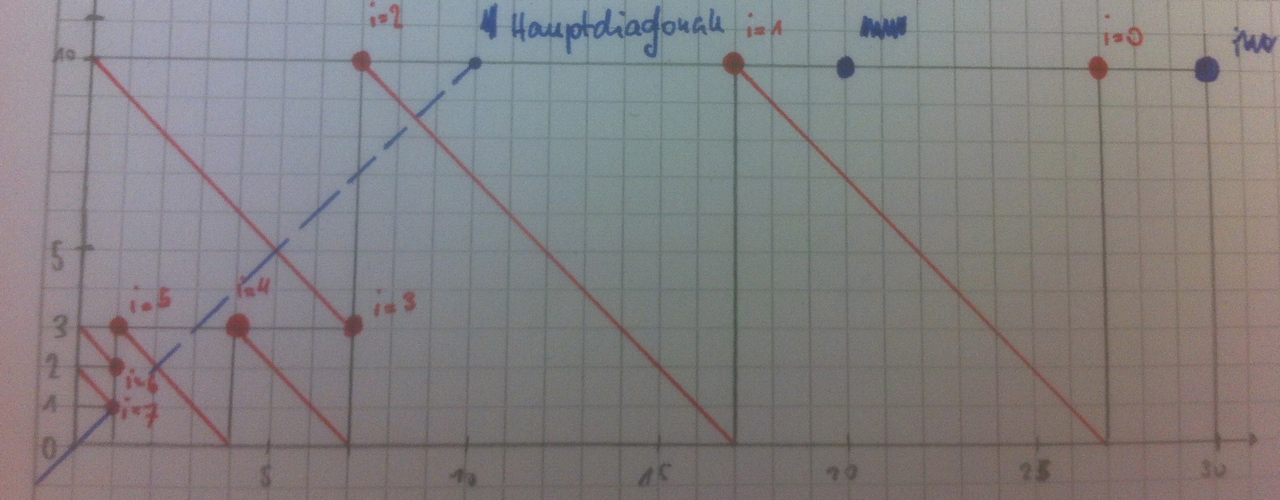
\includegraphics[scale=0.4]{euklid.png} \\
\\
\Bold {Regel e}: b = a * c + d $\Ra$ b gcd c = c gcd d \\
\\
b gcd c = c gcd (b - ac) Setze a = 1 \\
x gcd y = y gcd (x - y) \\
gcd(x,y) = gcd(y, x-y) \\
gcd(x,y) = gcd (x-y, y) : Korollar zu Regel e \\
\\
\Bold {Algo:} \\
Algo terminiert. Sei n Anzahl Iterationen. Dann gcd(bc) = $x_n$ oder $y_n$ (beides richtig) \\
$(x_0, y_0) = b, c$ \\
$i : = 0 $ \\
\Bold {while} $x_i \neq <_i$ \Bold {do} \\
	\Bold {if}  $x_i<y_i$ \Bold {then}
	$(x_i+1,y_i-1) = (x_i - y_i, y_i)$ \\
	\Bold {else} \\
	$(x_i+1,y_i-1) = (x_i,  y_i - x_i)$ \\
	\Bold {endif} \\
	i := i+1 \\
\Bold {end}

\subsection{Erweiterter Euklid}

\Bold {Satz:} \\
\begin{tabular}{l c l}
	$r_{-2} \underbrace{=}_{A}$ a & & $r_{-1} \underbrace{=}_{B}$ b\\
	$p_{-2} \underbrace{=}_{C}$ 0 & X & $p_{-1} \underbrace{=}_{D}$ 1 \\
	$q_{-2} \underbrace{=}_{E}$ 1 & & $q_{-1} \underbrace{=}_{F}$ 0 \\
\end{tabular} \\
i := 0 \\ \\
\Bold {while} $r_{i-1} \underbrace{>}_{G} 0$ \Bold {do} \\
\Bold {berechne} $c_i$ und $r_i$ mit $r_{i-2} \underbrace{=}_{H} c_i * r_{i-1} + r_i \wedge 0 \underbrace{\leq}_{I} r_i \underbrace{<}_{J} r_{i-1}$ \\
$p_i \underbrace{=}_{K} c_i * p_{i-1} + p_{i-2}$ \\
$q_i \underbrace{=}_{L} c_i*q_{i-1} + 1_{i-2}$ \\
$i:=i+1$ \\
\Bold {end} \\ 
\\
Seien a, b : $\NN$. \\
Dann gibt es Zahlen $x,y : \ZN$ mit $x*a + y*b =$ gcd(a,b). \\
Wir konstruieren diese Zahlen durch erteiterten Euklidschen Algorithmus. 
\begin{itemize}
	\item[1)] $r_{n-1} =gcd(a,b)$ 
	\item[2)] $p_n$ $gcd(a,b) = a$
	\item[3)] $q_n$ $gcd(a,b) = b$
	\item[4)] $a * \frac{q_{n-1}}{(-1)^{n-1}} + b * \frac{p_{n-1}}{(-1)^n}=gcd(a,b)$
\end{itemize}

\begin{tabular}{c c c c c l}
	i & $r_i$ & $c_i$ & $p_i$ & $q_i$ & \\
	-2 & 654 & & 0 & 1 & \\
	-1 & 444 & & 1 & 0 & \\
	0 & 210 & 1 & 1 & 1 & =b \\
	1 & 24 & 2 & 3 & 2 & = 210 \\
	2 & 18 & 8 & 25 & 17 & = 24 \\
	3 & 6 & 1 & 28 & 19 & = 18 \\
	4 & 0 & 3 & 109 & 74 & = 0 
\end{tabular} \\
\\
\Bold {Beweis} \\
Es gibt offensichtlich $n:\NN$ mit $r_n=0 \wedge (\forall i | 0 \leq i < n : r_i > 0)$ \\
Invarianten f\"ur alle $i : 0 \leq i \leq n+1$
\begin{itemize}
	\item[$I_1$:] ged($r_{i-2}$,$r_{i-1}$) = ged(a,b) 
	\item[$I_2$:] $p_{i-2} * r_{i-1} + p_{i-1} * r_{i-2} = a$
	\item[$I_3$:] $q_{i-2} * r_{i-1} + q_{i-1} * r_{i-2} = b$
	\item[$I_4$:] $q_{i-2} * p_{i-1} - q_{i-1} * p_{i-2} = (-1)^{i-1}$
\end{itemize}
\Bold {Beispiel $I_2$:}
\begin{description}
	\item[Induktionsanfang] \hfill \\
		$i=0, p_{-2} * r_{-1} + p_{-1} * r_{-2}$ \\
		$= <C, B, D, A>$ \\
		$0 * b + 1 + a$ \\
		$=<Arith>$ \\
		$a$
	\item[Induktionsschritt] \hfill \\
		zu zeigen: $I_2(i) \wedge r_{i-1} > 0 \Ra I_2(i+1)$ f\"ur alle i mit $0 \leq i \leq n$. \\
		Sei n eine $\NN$ mit $0 \leq i \leq n$ \\
		\\
		Annahme: es gibt $I_2(i) \wedge r_{i-1} > 0$ \\
		zu zeigen: es gibt $I_2(i+1)$ \\
		\\
		$p_{(i+1)-2} * r_{(i+1)-1} + p_{(i+1)-1} * r_{(i+1)-2}$ \\
		$= <Arith>$ \\
		$p_{i-1} * r_i + p_i * r_{i-1}$ \\
		$= <H, < >$ \\
		$p_{i-1} * (r_{i-2} - c_i * r_{i-1}) +(c_i * p_{i-1} + p_{i-2}) *r_{i-1}$ \\
		$= <Arith>$ \\
		$p_{i-1} * r_{i-2} + p_{i-2} * r_{i-1}$ \\
		$= <Annahme>$ \\
		a \\
		\\
		Es gilt insbesondere: $p_n * r_{n-1} + p_{n-1} * \overbrace{r_n}^{0}=a$  \\
		$p_n * gcd(a,b)=a \ra (2)$
\end{description}
\end{document}